
\ifdefined\pdfminorversion
  \pdfminorversion=7
\fi
\ifdefined\pdfsuppresswarningpagegroup
  \pdfsuppresswarningpagegroup=1
\fi

\documentclass[journal]{IEEEtran}

\usepackage{cite}
\usepackage{amsmath,amssymb,amsfonts}
\usepackage{graphicx}
\usepackage{booktabs}
\usepackage{multirow}
\usepackage{array}
\usepackage{url}
\usepackage{balance}
\usepackage[T1]{fontenc}

\newcommand{\ali}{\mathrm{ALI}}
\newcommand{\argmax}{\operatorname*{arg\,max}}
\newcommand{\jtwo}{J2}
\newcommand{\dbten}{DB10/MeganePro}

\begin{document}

\title{Agency-Budgeted Policy Evaluation for Myoelectric Prosthetic Grasping Under Distribution Shift: An Offline Open-Data Benchmark}

\author{Daniel~Choi, Andrew~Choi, Cordelia~Yip, Benjamin~Funk, Quan~Lam, and Junho~Park%
\thanks{Daniel Choi, Andrew Choi, Cordelia Yip, Benjamin Funk, Quan Lam, and Junho Park are with the University of Calgary, Calgary, AB, Canada.}
\thanks{Corresponding author: Junho Park (email: junho.park@ucalgary.ca).}}

\markboth{IEEE Transactions on Neural Systems and Rehabilitation Engineering,~Vol.~XX, No.~X, 2026}{D. Choi \MakeLowercase{\textit{et al.}}: Agency-Budgeted Policy Evaluation Under Distribution Shift}

\maketitle

\begin{abstract}
For upper-limb myoelectric prostheses, shared autonomy is not only an intent-decoding problem; it is also a rehabilitation-engineering policy problem: when may contextual assistance change a command implied by the user's sEMG branch? We introduce \jtwo, an offline open-data benchmark for agency-budgeted intervention policies under distribution shift. Dataset-specific user and assistive decoders produced calibrated posterior traces; a shared policy layer compared user-only, assist-only, confidence blending, confidence gating, SetACSA-style, and agency-margin policies. \dbten was the primary claim-bearing, amputee-relevant benchmark, with Hyser and CEMHSEY used as external high-density EMG robustness checks. In DB10, the assistive branch used an annotated object-context proxy rather than an end-to-end perception system, so results are offline policy-layer stress tests. Inference was performed at subject, session, or day level rather than window level. On the two primary DB10 families, user-only active macro-F1 was 0.081 in amputee leave-one-subject-out and 0.088 in mixed-to-amputee evaluation. Agency-margin at $\tau=0.20$ reached 0.658 and 0.694, while active risk-coverage AUC decreased from 0.890 to 0.254 and from 0.879 to 0.189. Against matched SetACSA, low-to-middle budgets ($\tau=0.02$, 0.05, 0.10) improved active macro-F1 and active risk-coverage in both primary DB10 families. A stronger exact-budget confidence audit found no universal fixed $\tau$ across DB10, Hyser, or CEMHSEY: confidence thresholds often improved DB10 active performance, whereas agency-margin reduced decoder-relative ALI. \jtwo therefore supports a reproducible performance--agency frontier, not an online-control claim, a perceived-agency claim, or a universal fixed operating point.
\end{abstract}

\begin{IEEEkeywords}
Myoelectric prostheses, shared autonomy, electromyography, distribution shift, selective prediction, calibration, rehabilitation engineering, open-data benchmark.
\end{IEEEkeywords}

\section{Introduction}
\IEEEPARstart{M}{yoelectric} prosthetic grasp control is commonly framed as intent decoding: estimate the intended grasp from surface electromyography (sEMG), increasingly with contextual information about the task or environment. This framing has produced major open resources for non-invasive hand-grasp and gesture recognition \cite{Atzori2014Ninapro,Cognolato2020MeganePro,Jiang2021Hyser,Jiang2023HyserPhysioNet,Yang2025CEMHSEY,Pradhan2022GRABMyo,Jiang2024GRABMyoPhysioNet}. It has also exposed a translation gap: offline classifier accuracy does not specify when an assistive system should alter the command selected by the user's myoelectric branch \cite{Jiang2012Focus,Scheme2011Selective}.

That gap becomes consequential under distribution shift. A decoder may behave differently for held-out amputee participants, for mixed able-bodied/amputee training evaluated on amputee participants, or across recording days in high-density EMG. An assistive branch can raise apparent performance by intervening frequently, whereas a conservative policy may preserve the user branch while leaving correctable errors unchanged. The relevant evaluation question is therefore whether assistance improves task performance within a declared intervention and agency-loss budget.

This paper introduces \jtwo, an offline open-data benchmark for policy-layer shared autonomy in myoelectric prosthetic grasping. \jtwo separates dataset-specific decoding from the intervention policy: each dataset retains its feature spaces, split definitions, label vocabulary, and calibration procedure, while a common policy layer decides whether the assistive estimate should affect the final command. This design supports policy comparisons across heterogeneous datasets without treating them as a single prosthetic task.

The novelty in \jtwo is therefore not a new grasp decoder, a new sensor dataset, or an online controller. It is the shared decision object between calibrated user and contextual branches: a reproducible test of how much decoded user preference a policy spends to obtain active-grasp performance under amputee-relevant distribution shift. This makes the benchmark a rehabilitation-engineering software-control contribution for myoelectric assistive devices rather than a generic machine-learning benchmark.

The primary dataset is \dbten, a multimodal prosthetic grasp dataset collected from able-bodied and transradial amputee participants and designed around sEMG, gaze, visual, inertial, and behavioral information \cite{Cognolato2020MeganePro}. In \jtwo, DB10 is used as an offline annotated context-assisted benchmark: the assistive branch uses an annotated object-context proxy rather than an end-to-end perception system. Hyser and CEMHSEY provide external robustness checks for two-day and 11-day high-density EMG shift \cite{Jiang2021Hyser,Jiang2023HyserPhysioNet,Yang2025CEMHSEY}. GRABMyo is retained as supplementary support \cite{Pradhan2022GRABMyo,Jiang2024GRABMyoPhysioNet}.

The contribution is threefold. First, \jtwo defines a policy-layer evaluation object for myoelectric shared autonomy: calibrated user and assistive posterior traces are converted into executed commands under declared intervention and decoder-relative agency-loss budgets. Second, it introduces a matched-budget evaluation suite with ALI, risk-coverage metrics, matched SetACSA-style comparisons, confidence-gate comparators, exact-budget confidence audits, and secondary timing analyses. Third, it reports a DB10-centered result in which agency-margin improves over matched SetACSA at selected low-to-middle budgets, while exact-budget confidence thresholding exposes a performance--agency frontier rather than a universal fixed operating point.

\section{Related Work and Benchmark Position}
\subsection{Open EMG and Prosthetic Grasp Data}
Open datasets are essential for reproducible prosthetic-control methodology. NinaPro established large open sEMG resources for non-invasive prosthetic movement recognition \cite{Atzori2014Ninapro}. DB10/MeganePro extends this line with multimodal grasp data, including sEMG, visual and gaze streams, inertial measurements, and participant metadata for 30 able-bodied and 15 transradial amputee participants \cite{Cognolato2020MeganePro}. Prior DB10/MeganePro analyses showed that contextual information can improve offline grasp-type classification \cite{Cognolato2022EyeVision,Wang2022VisionSEMG}. \jtwo uses the same dataset family for a different question: not whether context improves recognition, but whether a contextual estimate should be allowed to change the user-decoded command under an explicit authority budget.

Hyser and CEMHSEY address a different need: robust high-density EMG evaluation over session or day changes. Hyser contains 256-channel forearm HD-sEMG from 20 subjects recorded twice on separate days, with a 34-gesture pattern-recognition subset and additional force-related subsets \cite{Jiang2021Hyser,Jiang2023HyserPhysioNet}. CEMHSEY contains 320-channel HD-sEMG collected across 11 consecutive days, including a GRASP subset with 13 participants and seven grasp classes \cite{Yang2025CEMHSEY}. GRABMyo provides 43 participants, three sessions, and 17 gestures for gesture recognition and biometrics \cite{Pradhan2022GRABMyo,Jiang2024GRABMyoPhysioNet}. These datasets are not interchangeable with DB10; instead, they provide stress tests for whether the same policy layer behaves coherently under different EMG shifts.

\subsection{From Decoder Accuracy to Policy-Layer Evaluation}
Myoelectric control has long used pattern recognition, time-frequency features, and classifier-based rejection mechanisms \cite{Englehart1999TimeFrequency,Scheme2011Selective}. Robustness concerns such as electrode displacement, day-to-day change, force variation, and nonstationary signal structure motivate evaluation beyond within-session accuracy \cite{Hargrove2006Electrode,Jiang2012Focus}. Selective classification and modern selective prediction formalize a related idea: a model should sometimes abstain or defer when confidence is insufficient \cite{Scheme2011Selective,Geifman2019SelectiveNet}. Calibration methods such as temperature scaling are also relevant because policy decisions based on probability margins can fail when probabilities are miscalibrated \cite{Guo2017Calibration}.

\jtwo adapts these ideas to a prosthetic shared-autonomy decision object. The policy does not merely abstain; it decides whether to leave the user-decoded action unchanged or replace it with an assistive candidate. Thus, a confidence threshold is a strong comparator, not a weak baseline. A policy that cannot outperform a matched confidence gate on performance may still be valuable if it uses less decoder-relative ALI, but that should be stated as a tradeoff rather than as universal dominance.

\subsection{Relation to Online Shared-Control Studies}
Online semi-autonomous prosthesis studies demonstrate that contextual sensing and user-system interaction can support practical assistance in live tasks \cite{Castro2022Depth}. Those studies are indispensable for translation, but they answer a different question from J2. J2 does not validate online control, hardware integration, haptic feedback, workload, trust, embodiment, or perceived agency. Its contribution is an offline, reproducible, open-data policy benchmark: given calibrated user and assistive traces under declared distribution shifts, how do intervention policies trade active-grasp performance against decoder-relative agency loss?

\section{Methods}
\subsection{Study Scope and Evidence Hierarchy}
The benchmark used only previously released datasets; no new participant data were collected. The evidence hierarchy was intentionally asymmetric. \dbten was the only primary, claim-bearing prosthetic grasp benchmark because it includes transradial amputee participants and multimodal grasp context. The two primary split families were amputee leave-one-subject-out (\texttt{db10\_amputee\_loso}) and mixed-to-amputee (\texttt{db10\_mixed\_to\_amputee}). The able-to-amputee family was retained as a boundary transfer stress test. Hyser and CEMHSEY tested whether the same policy audit behaved coherently under HD-sEMG day/session shift; they were external robustness checks, not substitutes for DB10 prosthetic-grasp evidence. GRABMyo was supplementary.

\begin{table*}[!t]
\centering
\caption{Prepared benchmark datasets and manuscript roles. Rows are from the frozen J2 audit used for the manuscript package. DB10 is the claim-bearing dataset; Hyser and CEMHSEY are external robustness checks; GRABMyo is retained as supplementary support. User/assistive feature dimensions were 96/190 for DB10, 1280/2048 for Hyser, 1600/2560 for CEMHSEY, and 160/256 for GRABMyo.}
\label{tab:datasets}
\footnotesize
\begin{tabular}{p{0.095\textwidth}p{0.30\textwidth}rrrrrp{0.17\textwidth}}
\toprule
Dataset & Role & Rows & Subjects & Sessions & Days & Labels & Assistive context mode \\
\midrule
DB10 & Primary; amputee-relevant multimodal grasp benchmark & 189,000 & 45 & 1 & 0 & 11 & annotated\_object\_proxy \\
Hyser & External two-day HD-sEMG robustness check & 40,340 & 20 & 2 & 2 & 34 &  \\
CEMHSEY & External 11-day HD-sEMG robustness check & 24,020 & 13 & 1 & 11 & 7 &  \\
GRABMyo & Supplementary robustness check & 76,755 & 43 & 3 & 3 & 17 &  \\
\bottomrule
\end{tabular}
\end{table*}



\subsection{Prepared Bundles and Audits}
Each dataset was converted into a prepared bundle containing user features, assistive features, labels, metadata, split identifiers, and provenance. Raw samples from different datasets were not pooled into a single classifier. The shared object across datasets was the policy layer applied to calibrated posterior traces. The frozen audit included prepared row counts, subject/session/day counts, label counts, and feature dimensions. DB10 contained 189{,}000 prepared rows across 45 subjects and 11 labels; Hyser contained 40{,}340 rows across 20 subjects, two sessions/days, and 34 labels; CEMHSEY contained 24{,}020 rows across 13 subjects, 11 days, and seven labels; GRABMyo contained 76{,}755 rows across 43 subjects, three sessions/days, and 17 labels.

DB10 requires special care. The assistive feature block in this benchmark is an annotated object-context proxy. The proxy should be interpreted as contextual evidence, not as an executed-grasp label supplied to the policy. It deliberately removes perception errors from this benchmark so that the evaluated object is the intervention policy rather than a combined perception-control stack. Consequently, DB10 gains estimate what the policy layer can do when contextual evidence is informative; they do not estimate the performance of a deployable camera, object detector, gaze pipeline, or embedded controller.

\subsection{Split Families}
DB10 used three split families. The amputee LOSO family trained and tested across amputee subjects with held-out amputee test subjects. The mixed-to-amputee family trained from mixed available data and tested on amputee participants. The able-to-amputee family tested a harder population-transfer boundary. Hyser used subject-level and within-subject day-shift families. CEMHSEY used a forward-day family in which later-day data were tested after earlier-day training. Inference was summarized at subject, session, or day level depending on dataset structure; window-level observations were not treated as independent inferential units.

\subsection{Decoders and Calibration}
Dataset-specific decoders produced user-branch and assistive-branch posterior probabilities. The canonical frozen manifest used multilayer perceptron or tree-based decoders depending on dataset and feature block. Calibration was performed before policy evaluation. Calibration is essential because confidence-gated policies and agency-margin policies depend on posterior magnitudes, and uncalibrated confidence can misrepresent correctness likelihood \cite{Guo2017Calibration}. The manuscript reports expected calibration error (ECE) as a diagnostic, but no claim depends on calibration alone.

\subsection{Policy Layer}
For each observation $i$, the user decoder produced a posterior vector $p_i^U(a)$ over actions $a \in \mathcal{A}$, and the assistive decoder produced $p_i^A(a)$. The user candidate was
\begin{equation}
    u_i = \argmax_{a \in \mathcal{A}} p_i^U(a),
\end{equation}
and the assistive candidate was
\begin{equation}
    s_i = \argmax_{a \in \mathcal{A}} p_i^A(a).
\end{equation}
The policy layer selected the final executed action $\hat{y}_i$.

Let $c_i^U=\max_a p_i^U(a)$, $c_i^A=\max_a p_i^A(a)$, and $I_i=\mathbb{1}\{\hat{y}_i\neq u_i\}$. User-only returned $u_i$ and assist-only returned $s_i$. Confidence blending selected $\argmax_a\{(1-\alpha)p_i^U(a)+\alpha p_i^A(a)\}$ with $\alpha\in\{0.25,0.50,0.75\}$. Plain confidence gating returned $s_i$ when $c_i^A\geq\gamma$ and otherwise returned $u_i$. SetACSA-style policies returned $s_i$ only when $p_i^A(s_i)>p_i^U(u_i)$ and $\ali_i(s_i)\leq\tau$. Agency-margin policies formed $\mathcal{C}_i(\tau)=\{a:\ali_i(a)\leq\tau\}$, selected the admissible action maximizing $p_i^A(a)$, and returned $u_i$ if no selected assistive action exceeded $p_i^U(u_i)$. These policies bracket policy-layer behavior rather than exhaust all possible EMG decoders or perception models, because every policy receives the same calibrated posterior traces within a dataset and split.

\subsection{Decoder-Relative Agency-Loss Index}
The term agency is used here in a restricted computational sense. ALI measures how much the executed command departs from the action preferred by the user decoder exposed to the policy. It does not infer the user's latent intention and is not a measure of perceived agency, embodiment, workload, trust, acceptance, or user preference. For an action $a$, we define
\begin{equation}
    \ali_i(a) = \max\left(0, p_i^U(u_i)-p_i^U(a)\right).
\end{equation}
Thus, the user-decoded action has zero ALI, and an assistive override incurs higher ALI when the user decoder strongly preferred a different action. For an agency budget $\tau$, the agency margin is
\begin{equation}
    m_i(a;\tau) = \tau - \ali_i(a).
\end{equation}
A candidate satisfying $m_i(a;\tau) \geq 0$ is within budget. Mean ALI is reported over executed actions.

\subsection{Matched and Exact-Budget Confidence Audits}
A central methodological risk in shared-autonomy benchmarking is an unfair comparator. A proposed policy can look better than a confidence threshold if it intervenes more often or if the threshold is poorly matched. J2 therefore uses two confidence-threshold audits.

The publication grid used $\tau\in\{0.02,0.05,0.10,0.15,0.20\}$. First, matched confidence thresholds selected one global threshold from observed assistive confidences plus endpoint values to approximate the agency-margin action-change rate. Second, the exact-budget audit used a denser threshold bank from up to 201 quantiles of $c_i^A$ plus endpoints and selected thresholds to minimize residual action-change budget gaps at the inferential-unit level. This audit is intentionally strong and oracle-style: it asks whether agency-margin remains preferable when a plain-confidence comparator is allowed to match the budget as closely as possible on evaluated traces. It does not establish a deployable validation protocol unless thresholds are selected prospectively from validation data.

\subsection{Metrics and Statistical Inference}
The primary active-task performance metrics were active macro-F1 and active risk-coverage AUC. Macro-F1 was computed over class labels with zero division set to zero; active macro-F1 excluded label 0 for DB10 and treated all labels as active for Hyser, CEMHSEY, and GRABMyo. Risk-coverage AUC summarized cumulative risk after sorting by decreasing coverage confidence; lower values indicate better selective performance. ECE used 15 equal-width confidence bins. Secondary metrics included balanced accuracy, intervention rate, mean ALI, decision timing, safe-episode rate, stable-safe episode rate, and final-correct rate.

Paired comparisons were performed over subject/session/day units rather than individual windows. Confidence intervals were computed from paired unit-level differences, and two-sided paired tests used the same unit summaries. Multiple comparisons were controlled using Holm correction within each comparison family and metric block. Results are reported as benchmark findings rather than clinical claims.

\section{Results}
\subsection{Validation Gates and Claim Boundaries}
The frozen benchmark audit first fixed which comparisons could support claims. As summarized in Fig.~\ref{fig:flow}, the same policy layer was applied after dataset-specific calibration and evaluated with unit-level inference. The audit passed the DB10 multimodal-direction check, the DB10 active-grasp performance floor, the DB10 primary pairwise significance gate against SetACSA at low-to-middle budgets, and the prepared-bundle checks for DB10, Hyser, CEMHSEY, and GRABMyo. The exact-budget audit later showed that no fixed $\tau$ was universally supported across DB10, Hyser, and CEMHSEY. The Results therefore treat DB10 as the claim-bearing dataset and the remaining datasets as robustness checks for a performance--agency frontier, not as evidence for a universal operating point.

\begin{figure*}[!t]
\centering
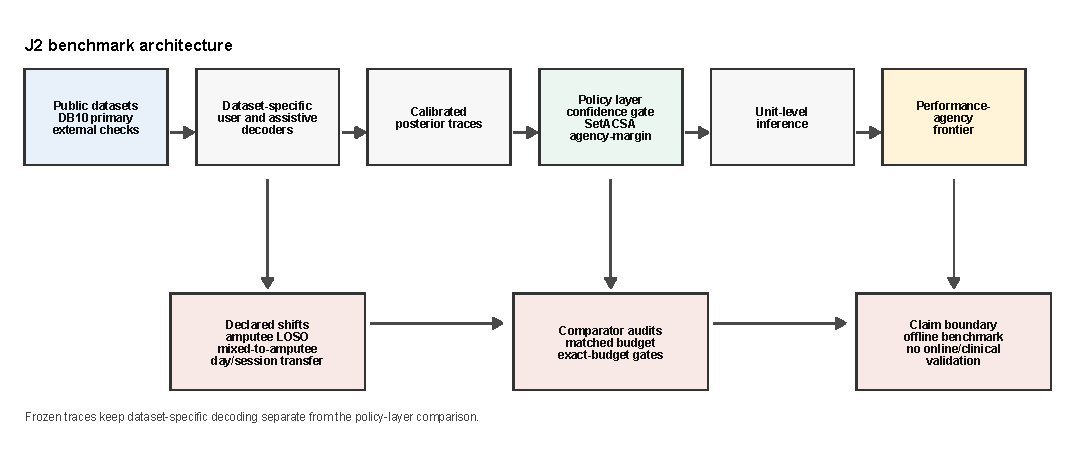
\includegraphics[width=0.98\textwidth]{figs/fig1_benchmark_flow.pdf}
\caption{J2 benchmark structure. Dataset-specific user and assistive decoders produce calibrated posterior traces, and a shared policy layer evaluates user-only, assist-only, confidence-based, SetACSA, and agency-margin decisions. Unit-level inference is performed over subject, session, or day units, depending on the split family.}
\label{fig:flow}
\end{figure*}

\subsection{DB10 Primary Results}
Table~\ref{tab:db10-main} and Fig.~\ref{fig:db10-frontier} show the DB10 primary frontier. In amputee LOSO and mixed-to-amputee evaluation, user-only active macro-F1 was 0.081 and 0.088, respectively. Agency-margin at $\tau=0.20$ reached 0.658 and 0.694, while active risk-coverage AUC decreased from 0.890 to 0.254 and from 0.879 to 0.189. These gains came with mean ALI of 0.053 and 0.048 and intervention rates of 0.799 and 0.785. Assist-only produced slightly higher active macro-F1 at higher mean ALI, whereas the matched confidence gate at $\tau=0.20$ used lower mean ALI but also lower active macro-F1. Thus, DB10 supports a frontier interpretation rather than a single dominant policy, especially because the assistive branch uses an annotated object-context proxy rather than a deployable perception stack.

\input{tables/db10_primary_table.tex}

\begin{figure*}[!t]
\centering
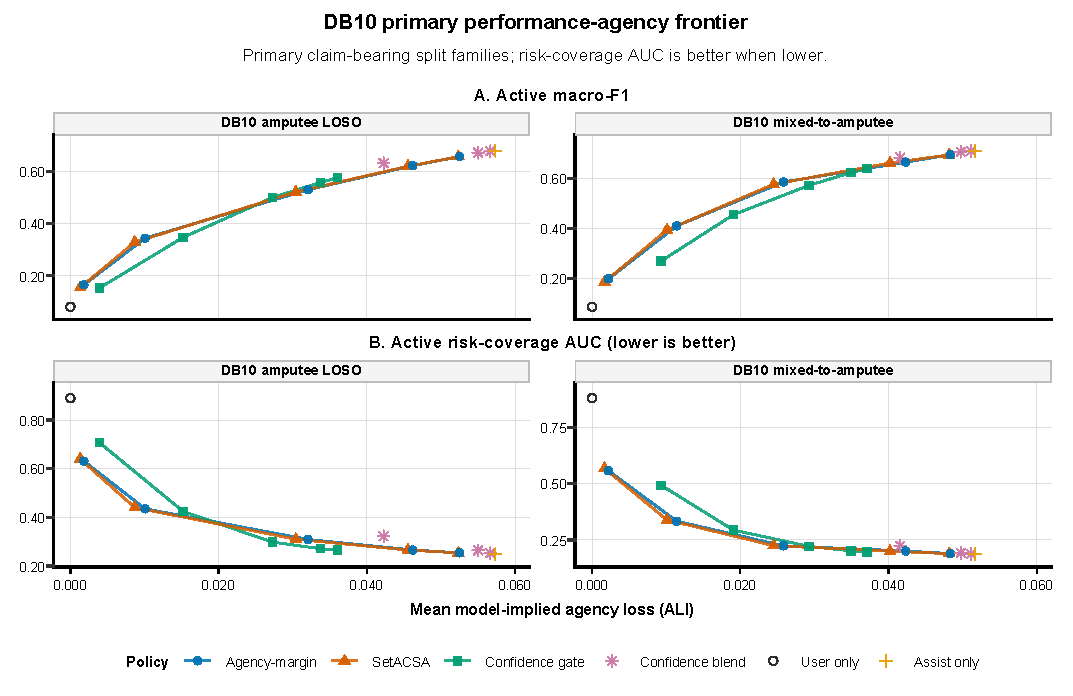
\includegraphics[width=0.98\textwidth]{figs/fig2_db10_frontier.pdf}
\caption{DB10 primary active-grasp performance--agency frontier. Points show active macro-F1 and active risk-coverage AUC versus mean model-implied agency loss in the two claim-bearing DB10 split families. Agency-margin and SetACSA trace similar budgeted trajectories; assist-only and confidence blending occupy higher-assistance regions, while confidence gates can reduce ALI with lower active macro-F1.}
\label{fig:db10-frontier}
\end{figure*}

\subsection{Agency-Margin Versus SetACSA}
Table~\ref{tab:setacsa-paired} and Fig.~\ref{fig:setacsa-paired} isolate the paired DB10 comparison between agency-margin and matched SetACSA. In both primary split families, $\tau=0.02$, 0.05, and 0.10 were Holm-beneficial for agency-margin on active macro-F1 and active risk-coverage AUC. Across those six rows, active macro-F1 gains ranged from 0.0089 to 0.0160, and active risk-coverage AUC changes ranged from -0.0101 to -0.0011, where negative values favor agency-margin. The effect is therefore modest but consistent, and the claim remains limited to low-to-middle DB10 budgets rather than generalized to all budgets or all datasets.

\begin{table*}[!t]
\centering
\caption{Paired DB10 agency-margin versus matched SetACSA comparison in the two primary amputee-relevant split families. For active macro-F1, positive estimates favor agency-margin. For active risk-coverage AUC, negative estimates favor agency-margin because lower AUC is better. All rows shown are Holm-beneficial in the frozen J2 audit.}
\label{tab:setacsa-paired}
\footnotesize
\begin{tabular}{llrrrr}
\toprule
Split family & $\tau$ & $\Delta$ Active F1 & 95\% CI & $\Delta$ Active risk AUC & 95\% CI \\
\midrule
DB10 amputee LOSO & 0.02 & 0.0109 & [0.0079, 0.0138] & -0.0095 & [-0.0124, -0.0066] \\
DB10 amputee LOSO & 0.05 & 0.0152 & [0.0111, 0.0188] & -0.0055 & [-0.0078, -0.0033] \\
DB10 amputee LOSO & 0.10 & 0.0090 & [0.0065, 0.0115] & -0.0013 & [-0.0020, -0.0006] \\
DB10 mixed-to-amputee & 0.02 & 0.0128 & [0.0099, 0.0155] & -0.0101 & [-0.0119, -0.0082] \\
DB10 mixed-to-amputee & 0.05 & 0.0160 & [0.0128, 0.0190] & -0.0057 & [-0.0076, -0.0039] \\
DB10 mixed-to-amputee & 0.10 & 0.0089 & [0.0065, 0.0114] & -0.0011 & [-0.0018, -0.0005] \\
\bottomrule
\end{tabular}
\end{table*}



\begin{figure*}[!t]
\centering
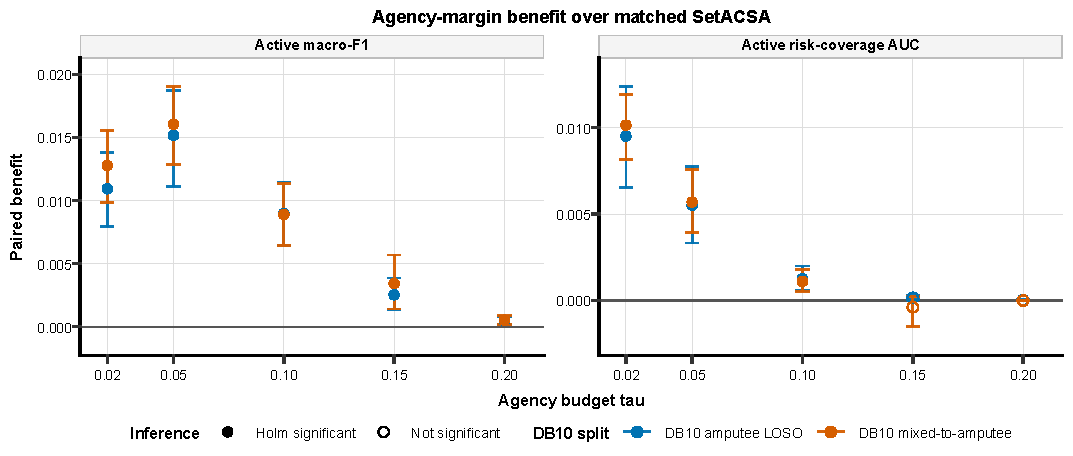
\includegraphics[width=0.88\textwidth]{figs/fig3_setacsa_pairwise.pdf}
\caption{Paired DB10 agency-margin minus matched SetACSA deltas across agency budgets. Positive active macro-F1 deltas favor agency-margin; negative active risk-coverage AUC deltas favor agency-margin because lower AUC is better. Error bars show paired 95\% confidence intervals over subject/session units, and filled markers indicate Holm-beneficial comparisons.}
\label{fig:setacsa-paired}
\end{figure*}

\subsection{Exact-Budget Confidence Audit}
Table~\ref{tab:exact-budget} and Fig.~\ref{fig:exact-budget} provide the central caveat. When plain confidence thresholds were selected from a dense bank to match the intervention budget, no fixed $\tau$ was universally supported across DB10, Hyser, and CEMHSEY. On DB10, agency-margin had 0/15 Holm-beneficial rows against exact-budget confidence thresholding for active macro-F1 and 0/15 for active risk-coverage AUC, but 15/15 Holm-beneficial rows for mean ALI; the worst residual budget gap was 0.0045. Hyser and CEMHSEY also favored agency-margin for mean ALI, but active performance was mixed. This audit converts the result from a method-superiority narrative into a performance--agency tradeoff.

\begin{table*}[!t]
\centering
\caption{Exact-budget confidence-threshold audit. Rows compare agency-margin against an exact-budget plain-confidence threshold selected from a dense threshold bank. Counts report Holm-beneficial rows for agency-margin out of all tested tau/split rows. The audit exposes a performance--agency frontier rather than a universal fixed operating point.}
\label{tab:exact-budget}
\footnotesize
\begin{tabular}{lrrrrrrr}
\toprule
Dataset & Split families & Universal $\tau$ & Fixed $\tau$ supported & Active F1 wins & Active risk AUC wins & Mean ALI wins & Worst budget gap \\
\midrule
DB10 & 3 & 0 & False & 0/15 & 0/15 & 15/15 & 0.0045 \\
Hyser & 2 & 0 & False & 1/10 & 6/10 & 10/10 & 0.0010 \\
CEMHSEY & 1 & 0 & False & 1/5 & 5/5 & 5/5 & 0.0016 \\
\bottomrule
\end{tabular}
\end{table*}



\begin{figure*}[!t]
\centering
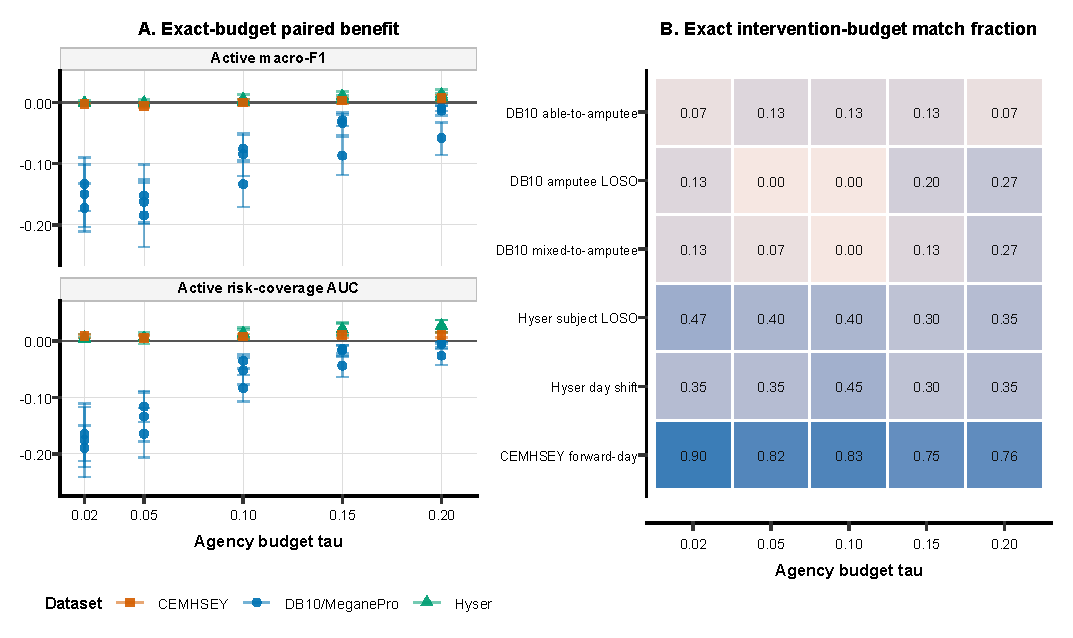
\includegraphics[width=0.88\textwidth]{figs/fig4_exact_budget_audit.pdf}
\caption{Exact-budget confidence-threshold audit. Panel A summarizes paired agency-margin benefit relative to exact-budget confidence thresholds across datasets and agency budgets. Panel B shows the fraction of rows in which the confidence-threshold bank exactly matched the requested intervention budget. DB10 favors agency-margin on mean ALI but not on active macro-F1 or active risk-coverage AUC, supporting a performance--agency frontier rather than a universal fixed $\tau$.}
\label{fig:exact-budget}
\end{figure*}

\subsection{External Robustness: Hyser and CEMHSEY}
Table~\ref{tab:external} and Fig.~\ref{fig:external-frontier} extend the same policy-layer audit to high-density EMG day/session shifts. On Hyser, agency-margin at $\tau=0.20$ gave small active macro-F1 gains over user-only in both subject LOGO (0.325 to 0.342) and day-shift evaluation (0.386 to 0.432). Confidence blending achieved higher active macro-F1 on Hyser but at higher mean ALI. On CEMHSEY, agency-margin improved active macro-F1 from 0.578 to 0.650 and active risk-coverage AUC from 0.258 to 0.230 with mean ALI of 0.015, whereas confidence blending reached 0.670 and 0.223 at mean ALI of 0.035. These datasets support the robustness of the policy-layer frontier pattern, but they are not prosthetic clinical validation.

\input{tables/external_table.tex}

\begin{figure*}[!t]
\centering
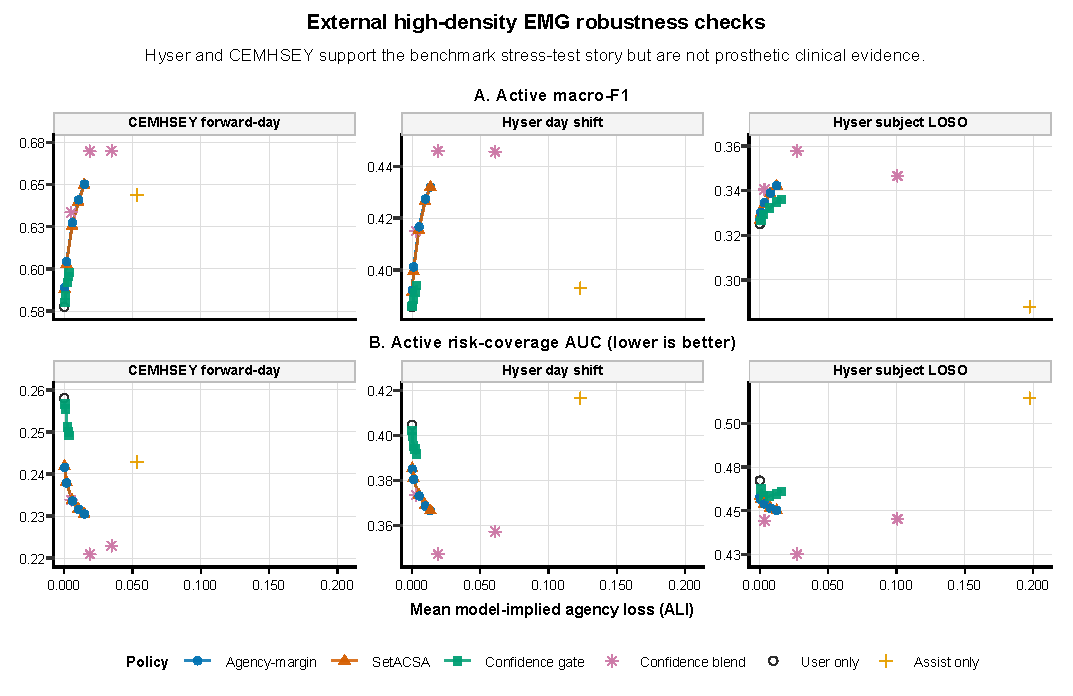
\includegraphics[width=0.98\textwidth]{figs/fig5_external_robustness.pdf}
\caption{External high-density EMG robustness frontiers for Hyser and CEMHSEY. Points show active macro-F1 and active risk-coverage AUC versus mean model-implied agency loss under day/session shift. These datasets test whether the policy-layer frontier pattern transfers beyond DB10, but they are not prosthetic clinical validation datasets.}
\label{fig:external-frontier}
\end{figure*}

\subsection{Timing and Earliest-Safe Behavior}
Fig.~\ref{fig:earliest-safe} reports DB10 timing as a secondary offline diagnostic. Across the two primary split families, larger agency budgets increased the stable-safe episode rate and reduced the median earliest stable-safe time for agency-margin and SetACSA. Confidence gating generally reached earlier stable-safe times at comparable budgets, but with lower stable-safe episode rates. These summaries indicate whether a policy's offline gains appear only at late decision points or can emerge earlier within an episode; they do not validate online shared-control timing, user adaptation, or perceived safety.

\begin{figure*}[!t]
\centering
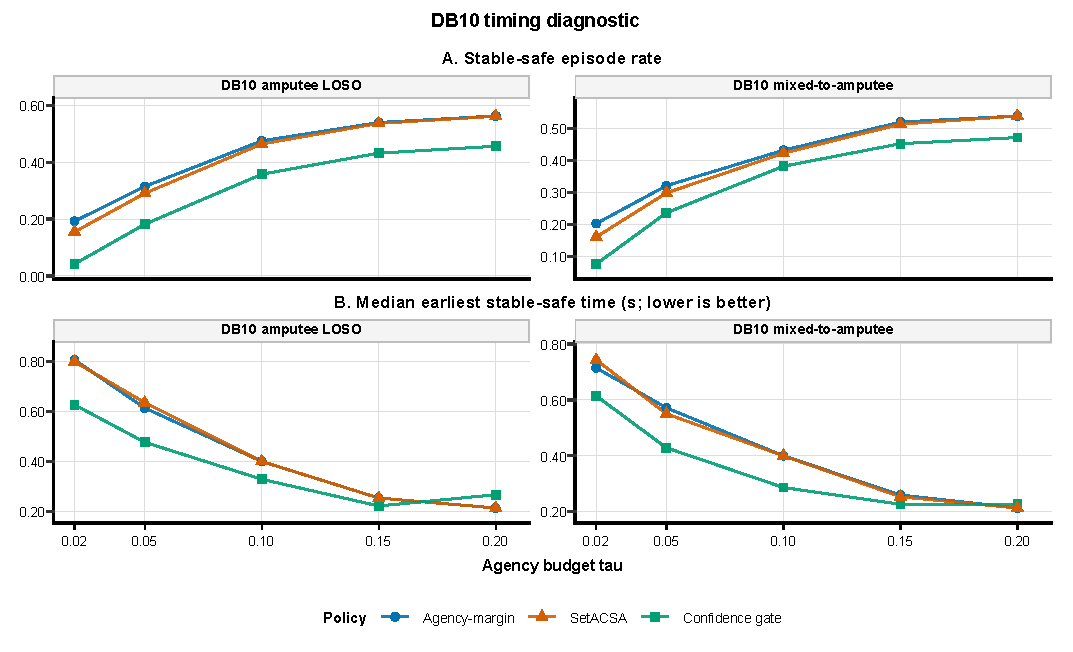
\includegraphics[width=0.92\textwidth]{figs/fig6_db10_earliest_safe.pdf}
\caption{DB10 offline timing diagnostic. Panel A reports stable-safe episode rate, and Panel B reports median earliest stable-safe time in seconds, where lower time is better. These prepared-trace summaries are secondary diagnostics and do not validate online shared-control behavior, user adaptation, or perceived safety.}
\label{fig:earliest-safe}
\end{figure*}

\section{Discussion}
\jtwo frames assisted myoelectric grasp evaluation as a policy-layer problem. The main result is a tradeoff, not universal superiority of agency-margin. In DB10, agency-margin outperformed SetACSA at low-to-middle budgets in the two primary amputee-relevant families. Exact-budget confidence thresholding then showed that a simple confidence gate can often achieve higher active performance when intervention rates are closely matched, while agency-margin lowers decoder-relative agency loss. The benchmark therefore identifies when a policy is a method improvement and when it is one point on a performance--agency frontier.

From a TNSRE scope perspective, the practical output is an auditable preclinical gate for assistive-device software: before a shared-autonomy policy is tested in hardware or with users, it should disclose how often it overrides the myoelectric branch, how much decoder-relative agency loss it incurs, and whether its claimed gains survive matched confidence-threshold comparators. That gate is directly tied to EMG-based prosthetic control even though the present evidence remains offline.

ALI should be read as a conservative policy diagnostic. It uses the user decoder's posterior preference as the reference and assigns cost to deviations from that preference. This makes ALI computable offline and comparable across policies, but it remains decoder-relative. If the user decoder is wrong or poorly calibrated, ALI is not a measure of perceived agency or true user preference; it only quantifies how far the executed command moved from the exposed user branch.

The DB10 annotated object-context proxy is useful because it isolates policy behavior when contextual assistance is informative. It is also a major boundary condition. The benchmark does not validate perception, camera placement, or hardware control. The separation between user-only and context-assisted results should therefore be interpreted as an offline policy stress test, not as evidence that the same gains would transfer directly to a deployed prosthesis.

Hyser and CEMHSEY broaden the stress test to high-density EMG day/session shifts. Their role is robustness support, not claim replacement. Consistency across DB10, Hyser, and CEMHSEY means that the policy-layer audit can be applied across heterogeneous EMG benchmarks; it does not mean that the same operating point, sensor configuration, or clinical behavior transfers across datasets.

\section{Limitations}
This study is offline. It does not test a prosthetic hand, online adaptation, haptic feedback, user training, task completion time in real manipulation, or subjective experience. It does not measure perceived agency, embodiment, trust, workload, comfort, or acceptance. ALI is model-implied and decoder-relative; a low-ALI policy should therefore be described as less disruptive relative to the user decoder, not as more acceptable, trusted, or embodied by the user.

The DB10 assistive branch uses annotated object context. That design is appropriate for an offline benchmark but not for deployment. A future online system would require a prospectively evaluated perception pipeline, user interaction model, and safety analysis. The exact-budget confidence audit is also partly diagnostic: if exact thresholds are selected using test-unit distributions, they should be read as an oracle-style fairness stress test rather than as a deployable calibration protocol.

Finally, the benchmark uses prepared features and canonical decoders. Better decoders, alternative calibration, subject-specific adaptation, additional sensor streams, or deployable perception modules could move the frontier. J2 is therefore a reproducible policy-layer baseline rather than a search over all possible EMG decoders, perception models, adaptive controllers, or clinical operating points.

\section{Conclusion}
\jtwo provides an offline open-data benchmark for agency-budgeted shared autonomy in myoelectric prosthetic grasping under distribution shift. In the primary DB10 amputee-relevant settings, agency-margin policies improve over matched SetACSA at selected low-to-middle budgets and produce large offline active-grasp gains relative to user-only decoding; these DB10 gains rely on an annotated object-context proxy in the assistive branch. Exact-budget confidence thresholding, however, shows that no universal fixed $\tau$ is supported across the audited datasets and that active performance can trade against decoder-relative ALI. The supported claim is therefore a transparent performance--agency frontier for future benchmark evaluation, not a deployable controller, clinical outcome, perceived-agency result, or universal method-superiority claim.

\section*{Data and Code Availability}
All datasets analyzed in this study are public resources and should be obtained from their original repositories. The manuscript package does not redistribute raw data. Code, configuration files, split and benchmark manifests, frozen aggregate outputs, figure-generation scripts, and manuscript source are available at \url{https://github.com/danielchoi0315/j2-agency-benchmark}.

\section*{Ethics Statement}
This study analyzed previously released public datasets and collected no new human-participant data. Dataset-specific ethics approvals and informed-consent procedures are reported in the original dataset publications and repositories \cite{Cognolato2020MeganePro,Jiang2021Hyser,Jiang2023HyserPhysioNet,Yang2025CEMHSEY,Pradhan2022GRABMyo,Jiang2024GRABMyoPhysioNet}. No clinical trial, online prosthesis test, or human-subject intervention was conducted. Any future online or hardware study derived from J2 would require prospective ethics review, participant consent, device-safety procedures, and explicit monitoring of perceived agency, workload, trust, comfort, and task-level risk.

\section*{Supplementary Material}
The supplementary file submitted with this manuscript reports additional matched-budget ablations and external timing diagnostics.

\balance
\bibliographystyle{IEEEtran}
\bibliography{references}

\end{document}

